\paragraph{D-MOSFET} \mbox{} \\
D-MOSFET kalles depletion (nedbryting) mosfet fordi det n-dopede materialet blir
positivt ladet og derfor \emph{brytes ned}.
Se på den visuelle likheten mellom dmosfet og emosfet så forstår du hva
jeg mener.
\\\\
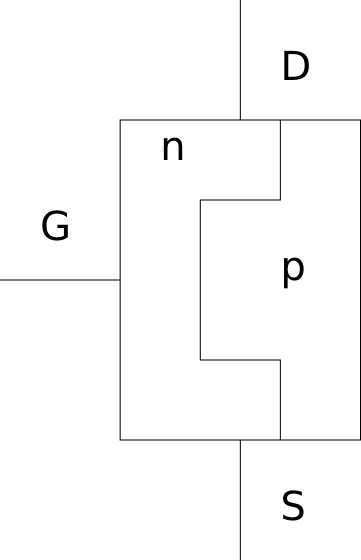
\includegraphics[width=0.5\textwidth]{./img/dmosfet}
\\\\
Mellom Gate og n-type er det en isolator som ikke er tegnet i inn.
\\\\
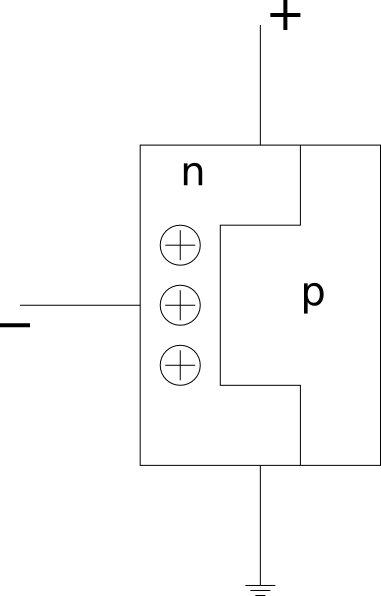
\includegraphics[width=0.5\textwidth]{./img/dmosfet-depleted}
\\\\
Her ser vi at n-materialet har mistet elektroner og er derfor brutt
ned (depleted).



\paragraph{E-MOSFET} \mbox{} \\
Enhancement (legge til) mosfet fungerer omtrent motsatt fra en dmosfet.
Istedenfor at n-området brytes i to, er den allerede brutt i to, men det kan
fylles igjen.
\\\\
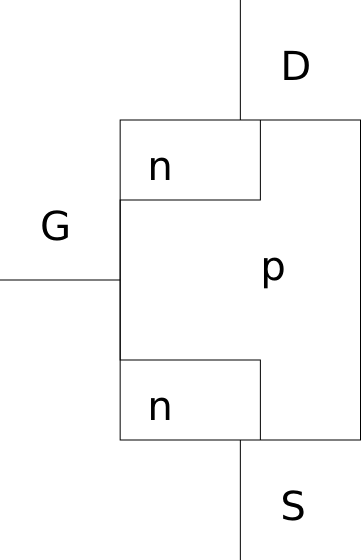
\includegraphics[width=0.5\textwidth]{./img/emosfet}
